% Figure: what CLIP does. Left: one image and five captions are embedded in one space; cosine scores differ little, the temperature softmax turns them into a sharp choice, and a caption with an extra wrong detail still scores close to the right one. Right: training fills a BxB matrix whose diagonal holds the true pairs.
% Design width ~168mm, height ~70mm.
\documentclass[border=0pt]{standalone}
\usepackage{amsmath,amssymb}
% Shared visual language for the figures of the book.
% Every figure in this directory loads this file so the chapter reads as one system.
% NOTE: no blank lines are allowed inside \tikzset{...} (a blank line emits \par
% and breaks key scanning).
\NeedsTeXFormat{LaTeX2e}
\ProvidesPackage{figstyle}[2026/10/21 Figure style for Free Energy to LLMs]

\RequirePackage{tikz}
\usetikzlibrary{arrows.meta,positioning,calc,fit,shapes.geometric,shapes.misc,%
  backgrounds,matrix,decorations.pathreplacing,decorations.markings,patterns.meta}

% ---------------------------------------------------------------- palette
% Same values as book/preamble/style.tex, prefixed with F.
\definecolor{FNavy}{HTML}{14324A}
\definecolor{FTeal}{HTML}{0E7490}
\definecolor{FSky}{HTML}{E7F5F8}
\definecolor{FOrange}{HTML}{D97706}
\definecolor{FAmber}{HTML}{FFF3D6}
\definecolor{FInk}{HTML}{1F2937}
\definecolor{FSlate}{HTML}{64748B}
\definecolor{FMist}{HTML}{F5F7FA}
\definecolor{FRose}{HTML}{9F1239}
\definecolor{FRoseMist}{HTML}{FFF1F2}

% ---------------------------------------------------------------- semantics
% Teal   = probability / model / data object
% Orange = training objective, cost, or the quantity moved through the system
% Navy   = neutral structure
% Slate  = secondary label or metadata
% Rose   = failure mode, hazard, masked-out region
\tikzset{
  % Lay figures out in millimetres.  A figure designed 168mm wide is included at
  % \textwidth, so its fonts appear at exactly the size written here.
  every picture/.style={x=1mm,y=1mm,font=\small,line cap=round,line join=round},
  % ---- block styles
  nbase/.style={draw,rounded corners=1.2pt,align=center,inner sep=2.4pt,%
    minimum height=7mm,text=FInk},
  nteal/.style={nbase,draw=FTeal,fill=FSky},
  norange/.style={nbase,draw=FOrange,fill=FAmber},
  nnavy/.style={nbase,draw=FNavy,fill=white},
  nsoft/.style={nbase,draw=FSlate!55,fill=FMist},
  nrose/.style={nbase,draw=FRose,fill=FRoseMist},
  ghost/.style={draw=none,fill=none,align=center,inner sep=1pt},
  plain/.style={draw=none,fill=none,align=center,inner sep=0pt},
  % ---- arrows
  ar/.style={-{Latex[length=1.7mm,width=1.35mm]},draw=FSlate,line width=0.75pt},
  ard/.style={ar,dashed},
  arteal/.style={ar,draw=FTeal},
  arorange/.style={ar,draw=FOrange},
  arrose/.style={ar,draw=FRose},
  thickar/.style={ar,line width=1.2pt},
  % ---- text roles
  ftitle/.style={font=\large\bfseries,text=FNavy,align=center},
  ptitle/.style={font=\small\bfseries,text=FNavy,align=center},
  ptitleo/.style={font=\small\bfseries,text=FOrange,align=center},
  lbl/.style={font=\scriptsize,text=FSlate,align=center,inner sep=1pt},
  lblt/.style={lbl,text=FTeal},
  lblo/.style={lbl,text=FOrange},
  lbln/.style={lbl,text=FNavy},
  lblr/.style={lbl,text=FRose},
  sub/.style={font=\scriptsize,text=FSlate!90,align=center,inner sep=1pt},
  monob/.style={font=\ttfamily\scriptsize,text=FInk,inner sep=1pt},
  mathb/.style={font=\small,text=FInk,inner sep=1pt},
  eqn/.style={font=\scriptsize,inner sep=1.5pt,text=FInk},
  % ---- decorations
  brace/.style={decorate,decoration={brace,amplitude=2.4pt},draw=FSlate,%
    line width=0.6pt},
  bracet/.style={brace,draw=FTeal},
  braceo/.style={brace,draw=FOrange},
  axis/.style={draw=FSlate!55,line width=0.6pt},
  guide/.style={draw=FSlate!45,line width=0.5pt,dashed},
  halolabel/.style={font=\scriptsize,text=FInk,fill=white,fill opacity=0.85,%
    text opacity=1,inner sep=1.4pt,align=center},
}

% Figure title above the drawing, anchored at the figure's top-left.
\newcommand{\figtitle}[2][0]{%
  \node[ftitle,anchor=north west,outer sep=0pt] at (#1,0) {#2};}

% Rounded panel behind a subgroup of nodes.
\newcommand{\figpanel}[3][]{%
  \node[draw=FSlate!35,fill=#3,rounded corners=2pt,inner sep=2.6mm,#1] {#2};}

\endinput

\begin{document}
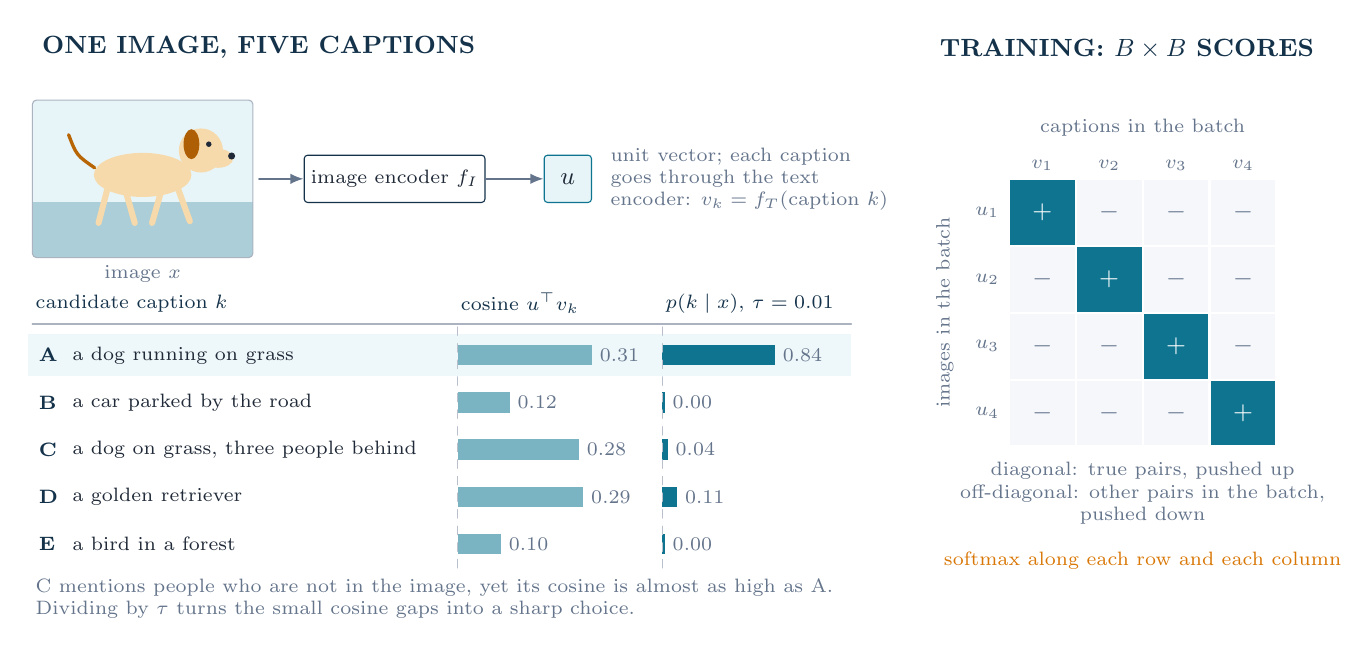
\begin{tikzpicture}
% ------------------------------------------------------- left: scoring captions
\node[ptitle,anchor=south west] at (2,68) {ONE IMAGE, FIVE CAPTIONS};
\begin{scope}
  \clip[rounded corners=1.5pt] (2,44) rectangle (30,64);
  \fill[FSky] (2,44) rectangle (30,64);
  \fill[FTeal!35] (2,44) rectangle (30,51);
  \fill[FAmber!80!FOrange] (16,54.5) ellipse (6.2 and 2.8);
  \draw[FAmber!80!FOrange,line width=2.2pt] (11.6,53) -- (10.4,48.4);
  \draw[FAmber!80!FOrange,line width=2.2pt] (13.8,52.6) -- (15,48.4);
  \draw[FAmber!80!FOrange,line width=2.2pt] (18.4,52.6) -- (17.2,48.4);
  \draw[FAmber!80!FOrange,line width=2.2pt] (20.4,53) -- (22,48.6);
  \draw[FOrange!85!black,line width=1.2pt] (9.9,55.4) .. controls (7.6,57) .. (6.6,59.6);
  \fill[FAmber!80!FOrange] (23.4,57.6) circle (2.8);
  \fill[FAmber!80!FOrange] (25.6,56.6) ellipse (1.9 and 1.2);
  \fill[FOrange!80!black] (22.2,58.4) ellipse (1.0 and 1.9);
  \fill[FInk] (24.4,58.4) circle (0.35);
  \fill[FInk] (27.3,56.9) circle (0.45);
\end{scope}
\draw[FSlate!55,rounded corners=1.5pt] (2,44) rectangle (30,64);
\node[lbl,anchor=north] at (16,43.4) {image $x$};
\node[nnavy,minimum width=22mm,minimum height=6mm,font=\scriptsize] (fi) at (48,54) {image encoder $f_I$};
\draw[ar] (30.8,54)--(fi.west);
\node[nteal,minimum width=6mm,minimum height=6mm,inner sep=0pt] (u) at (70,54) {$u$};
\draw[ar] (fi.east)--(u.west);
\node[lbl,anchor=west,align=left] at (75,54) {unit vector; each caption\\goes through the text\\encoder: $v_k=f_T(\text{caption }k)$};
% header row
\node[lbln,anchor=west] at (2,38.2) {candidate caption $k$};
\node[lbln,anchor=west] at (56,38.2) {cosine $u^\top v_k$};
\node[lbln,anchor=west] at (82,38.2) {$p(k\mid x)$, $\tau=0.01$};
\draw[axis] (2,35.6)--(106,35.6);
% rows: letter, caption, cosine, probability
\foreach \y/\l/\txt/\c/\p/\hl in {%
  31.6/A/{a dog running on grass}/0.31/0.84/1,%
  25.6/B/{a car parked by the road}/0.12/0.00/0,%
  19.6/C/{a dog on grass, three people behind}/0.28/0.04/0,%
  13.6/D/{a golden retriever}/0.29/0.11/0,%
  7.6/E/{a bird in a forest}/0.10/0.00/0}{%
  \ifnum\hl=1
    \fill[FSky!70] (1.4,{\y-2.7}) rectangle (106,{\y+2.7});%
  \fi
  \node[lbln,font=\scriptsize\bfseries,anchor=west] at (2.4,\y) {\l};%
  \node[font=\scriptsize,text=FInk,anchor=west,inner sep=0pt] at (7,\y) {\txt};%
  \fill[FTeal!55] (56,{\y-1.3}) rectangle ++({55*\c},2.6);%
  \node[lbl,anchor=west] at ({56.6+55*\c},\y) {\c};%
  \fill[FTeal] (82,{\y-1.3}) rectangle ++({max(0.3,17*\p)},2.6);%
  \node[lbl,anchor=west] at ({82.6+max(0.3,17*\p)},\y) {\p};%
}
\draw[guide] (56,4.6)--(56,35.2);
\draw[guide] (82,4.6)--(82,35.2);
\node[lbl,anchor=north west,align=left] at (2,3.6)
  {C mentions people who are not in the image, yet its cosine is almost as high as A.\\Dividing by $\tau$ turns the small cosine gaps into a sharp choice.};
% ------------------------------------------------------- right: training batch
\node[ptitle,anchor=south] at (141,68) {TRAINING: $B\times B$ SCORES};
\def\cx{126}\def\cy{20}\def\cs{8.5}
\foreach \j in {1,...,4}{%
  \node[lbl,anchor=south] at ({\cx+\cs*(\j-0.5)},{\cy+4*\cs+0.6}) {$v_{\j}$};%
  \node[lbl,anchor=east] at ({\cx-0.8},{\cy+\cs*(4.5-\j)}) {$u_{\j}$};%
}
\foreach \i in {1,...,4}{%
  \foreach \j in {1,...,4}{%
    \ifnum\i=\j
      \fill[FTeal] ({\cx+\cs*(\j-1)},{\cy+\cs*(4-\i)}) rectangle ++(\cs,\cs);%
      \node[font=\small\bfseries,text=white] at ({\cx+\cs*(\j-0.5)},{\cy+\cs*(4.5-\i)}) {$+$};%
    \else
      \fill[FMist] ({\cx+\cs*(\j-1)},{\cy+\cs*(4-\i)}) rectangle ++(\cs,\cs);%
      \node[font=\small,text=FSlate] at ({\cx+\cs*(\j-0.5)},{\cy+\cs*(4.5-\i)}) {$-$};%
    \fi
  }%
}
\foreach \g in {0,...,4}{%
  \draw[white,line width=0.8pt] ({\cx+\cs*\g},\cy)--({\cx+\cs*\g},{\cy+4*\cs});%
  \draw[white,line width=0.8pt] (\cx,{\cy+\cs*\g})--({\cx+4*\cs},{\cy+\cs*\g});%
}
\node[lbl,anchor=south] at ({\cx+2*\cs},{\cy+4*\cs+5}) {captions in the batch};
\node[lbl,rotate=90,anchor=south] at ({\cx-6.6},{\cy+2*\cs}) {images in the batch};
\node[lbl,anchor=north,align=center] at ({\cx+2*\cs},{\cy-1.6})
  {diagonal: true pairs, pushed up\\off-diagonal: other pairs in the batch,\\pushed down};
\node[lblo,anchor=north,align=center] at ({\cx+2*\cs},{\cy-13})
  {softmax along each row and each column};
\end{tikzpicture}
\end{document}
